\section{Annexe}
\label{theoretical}

This content is a synthesis of this course\cite{INF556} and other
information on the internet.

\paragraph{Motivation} Given a point set, find the underlying (homological) structures of
the data. First, let's consider a topological space, how do we determine
the homology structure of the space in a computational way.

\begin{definition}[$p$-simplex ($p\in\N$)]
  Let $V$ be some finite set (the vertices).
  A $p$-simplex $\sigma$ is the convex hull of $p+1$
  points $x_0, \ldots, x_p \in V$.
  We denote $\sigma = \conv\{x_0, \ldots, x_p\}$ a subset of $V$.
\end{definition}
\RM In practice, we simplify a topological space to its homology equivalence (thin
triangulation) without
losing the information we want (connected components, holes).

\begin{definition}[Face]
  A face of $\sigma$ is $\conv(S)$ where $S\subset\{x_0,\ldots, x_p\}$
\end{definition}

\begin{definition}[Simplicial complex]
  A simplicial complex $X$ is a finite collection of simplices s.t.
  $$
  \forall \sigma\in X, \forall \tau\subset\sigma, \tau\in X
  $$
\end{definition}

\begin{definition}[Chain space]
  The vectorial space of $k$-chains of a simplicial complex $X$ over a field $\K$ is defined by:
  $$
  C_k(X) := \left\{\sum_{i=1}^{\left|X_k\right|} \alpha_i \sigma_i: \alpha_i \in \mathbb{K}, \sigma_i \in X_k\right\}
  \simeq \K^{|X_k|}
  $$
  where $X_k = \{A\subset X : |A|=k+1\}$ the set of $k$-simplexes in $X$.
\end{definition}
\RM Let's work with $\K = \Z/2\Z$ so that we don't consider orientation.

\begin{definition}[$p$-chain]
  A $p$-chain is a subset of $p$-simplices in a simplicial complex $X$.
\end{definition}

\begin{definition}[Boundary operator]
  $$
  \begin{aligned}
  \partial_k: C_k(X) & \to C_{k-1}(X) \\
  \sigma=\{ v_0, \ldots, v_k \} & \mapsto \sum_{j=0}^k(-1)^j \underbrace{ \{v_0,\ldots,v_k \} \setminus \{v_j\}}_{\in X_{k-1}} \\
  \left(\lambda \sigma+\sigma^{\prime}\right) & \mapsto \lambda \partial_k \sigma+\partial_k \sigma^{\prime} \text{ (linear extension)}
  \end{aligned}
  $$
\end{definition}

\begin{lemma}
  $$
  \forall k, \partial_k \partial_{k+1} = 0
  $$
  \label{lem:pp0}
\end{lemma}

\begin{definition}[$k$-th homology group]
  \begin{itemize}
    \item $k$-cycles : $Z_k:=\Ker(\partial_k)$
    \item $k$-boundaries : $B_k:=\Im(\partial_{k+1})$
  \end{itemize}
  The $k$-th homology group of $X$ for the field $\K$ is the following quotient
  of vector spaces:
  $$
  H_k(X):={Z_k\over B_k}
  $$
  (well defined because of the Lemma~\ref{lem:pp0})
  The $k$-th Betti number $\beta_k = \mathrm{rank}(H_k)$.
\end{definition}
\RM The computational method is by Gauss elimination, we omit it here
because we later introduce a method to calculate barcodes which is more
powerful and uses Gauss elimination too.

Now, we are able to give the homology structure of a given topological space (simplicial complex).
Let's go back to the beginning, initially, we are only given a point set,
we may link the points in the set to form a simplicial complex.
The way in which we link the points change our view of the underlying structure.
The scale matters Figure~\ref{fig:scale}.

\begin{figure}[H]
  \centering
  \begin{tikzpicture}[scale=0.4]

  \coordinate (v1) at (0,0);
  \coordinate (v2) at (0,3);
  \coordinate (v3) at (3,0);
  \coordinate (v4) at (3,3);
  \draw (v1) -- (v2);
  \draw (v3) -- (v4);
  \draw (v1) -- (v3);

  \coordinate (w1) at (8+0,0);
  \coordinate (w2) at (8+0,3);
  \coordinate (w3) at (8+3,0);
  \coordinate (w4) at (8+3,3);
  \draw (w1) -- (w2);
  \draw (w3) -- (w4);
  \draw (w1) -- (w3);
  \draw (w2) -- (w4);
  \draw[->] (4,1.5) -- (7,1.5);

  \coordinate (u1) at (16+0,0);
  \coordinate (u2) at (16+0,3);
  \coordinate (u3) at (16+3,0);
  \coordinate (u4) at (16+3,3);
  \draw (u1) -- (u2);
  \draw (u3) -- (u4);
  \draw (u1) -- (u3);
  \draw (u2) -- (u4);
  \draw (u1) -- (u4);
  \draw[->] (12,1.5) -- (15,1.5);

  \coordinate (uu1) at (24+0,0);
  \coordinate (uu2) at (24+0,3);
  \coordinate (uu3) at (24+3,0);
  \coordinate (uu4) at (24+3,3);
  \draw (uu1) -- (uu2);
  \draw (uu3) -- (uu4);
  \draw (uu1) -- (uu3);
  \draw (uu2) -- (uu4);
  \draw (uu1) -- (uu4);
  \filldraw[fill=gray] (uu1) -- (uu4) -- (uu2);
  \draw[->] (20,1.5) -- (23,1.5);

  \foreach \vertex in {v1,v2,v3,v4,w1,w2,w3,w4,
  u1,u2,u3,u4,
  uu1,uu2,uu3,uu4}
    \fill (\vertex) circle (5pt);

  \coordinate (d) at (1.5,-0.5);
  \draw[->] ($(v1)+(d)$) -- node[left] {$H_1$} ++(0,-2) node[below] {$\K^0$};
  \draw[->] ($(w1)+(d)$) -- ++(0,-2) node[below] {$\K^1$};
  \draw[->] ($(u1)+(d)$) -- ++(0,-2) node[below] {$\K^2$};
  \draw[->] ($(uu1)+(d)$) -- ++(0,-2) node[below] {$\K^1$};

  \draw[->] (4, -2.75) -- node[above] {$0$}++(3,0);
  \draw[->] (12,-2.75) -- node[above] {$\begin{pmatrix}1\\0 \end{pmatrix}$}++(3,0);
  \draw[->] (20,-2.75) -- node[above] {$\begin{pmatrix}1 & 0 \end{pmatrix}$}++(3,0);
  
  \node at (13.5,-4.5) {\rotatebox{270}{$\simeq$}};
  \node at (13.5,-6) {$\I_{[2, \infty)} \oplus \I_{[3, 4)}$};

\end{tikzpicture}
  \caption{Filtration gives persistence module gives decomposition gives barcodes}
  \label{fig:tda_diagram}
\end{figure}

\begin{definition}[Filtration]
  A filtration over $T$ is a family $\F = (F_t)_{t\in T}$ of increasing topological spaces:
  $$
  \forall t, t^{\prime} \in T, t \leqslant t^{\prime} \Rightarrow F_t \subset F_{t^{\prime}}
  $$
\end{definition}

\begin{definition}[Persistence module]
  Let $\mathbb{K}$ be a given field. A persistence module over $T \subset \mathbb{R}$ is a family $\mathbb{V}=\left(V_t\right)_{t \in T}$ of $\mathbb{K}$-vector spaces
  endowed with linear application $v_t^{t^{\prime}}: V_t \rightarrow V_{t^{\prime}}$ induced by
  a filtration by being applied $H_k$ (e.g.\ Figure~\ref{fig:tda_diagram}).

  $\I_{[l, r)}$(the interval can be open/close at 2 ends) is an interval module with $T = [l, r)$,
  $(V_t)_t = (\K)_t$, $(v^{t'}_t) = (\id)$.
\end{definition}

\begin{theorem}[Decomposition theorem]
  A persistence module $\mathbb{V}$ can be decomposed as a direct sum of interval module
  in the following case (sufficient, not necessary):
  \begin{itemize}
    \item If $T$ is finite. [Gabriel, 72]
    \item When all the vector spaces $V_t$ are finite-dimensional. [Crowley-Boevey, 2012]
  \end{itemize}
  Furthermore, when it exists, the decomposition is unique (up to isomorphism and ordering of terms).
  See an example at Figure~\ref{fig:tda_diagram}
\end{theorem}

\RM Intuitively, the way to decompose is beginning from where a cycle occurs
and following the linear map until it diminishes and concluding an interval module;
the multiset of pairs of extremities of the intervals obtained by decomposition is called the \textbf{barcodes}
or the \textbf{persistence diagram}; to compute the decomposition, we do Gauss elimination (explained in the following).

\subsubsection{Algorithm to calculate the persistence diagram}

\paragraph{Input} A simplicial filtration, that is a filtration over a simplicial complex $K$ which verifies:
\begin{itemize}
  \item $T=\{1, \ldots, m\}$ (finite, so we have a decomposable filtration).
  \item $K_1=\{\sigma_1\}, K_m = K$
  \item $\forall t \in T, K_t$ is a simplicial complex,
  which is a sub-complex of $K_{t+1}$.
  \item We only add one simplex at each step,
  that is $K_{t+1} \backslash K_t=$ $\left\{\sigma_{t+1}\right\}$.
\end{itemize}

\begin{algorithm}
  \caption{Compute the barcodes corresponding to a simplicial filtration}
  \begin{algorithmic}
  \State M := the matrix of boundray operator $\partial$ =: $(c_0, \ldots, c_m)$
  \State $\mathrm{low}(j):=\left\{\begin{array}{l}\max \left\{i \mid M_{i j} \neq 0\right\} \\ 0 \text { if } M_{i j}=0 \text { for all } i\end{array}\right.$
  \For{$j = 1\ldots m$}
  \While{$\exists i<j$ s.t. $\mathrm{low}(i)=\mathrm{low}(j) \neq 0$}
  \State $c_j \gets c_j+c_i$ (Still working with $\K = \Z/2\Z$)
  \EndWhile
  \EndFor
  \State Barcodes are $\{(i, \max\{j \mid \mathrm{low}(j)=i\}) \mid c_i = 0\}$
  (1. This is a multiset 2. $\max$ return $\infty$ if empty 3. the set where we take max is of size at most 1)
  \end{algorithmic}
\end{algorithm}

\begin{proof}[Proof of validity]
Each $c_i = 0$ means the birth of a cycle (one plus for the dimension of the kernel).
Each $c_i \not= 0$ trivialize a cycle (one plus for the dimension of the image).
It remains to show that the pairing is right.

Consider a $c_j \not= 0$, $c_j = e_{l_1} + \cdots + e_{l_k}~(0\le l_1 < \cdots < l_k < j)$.
Note that $\partial_d (\sigma_{l_1} + \cdots + \sigma_{l_k}) = 0$ (Lemma~\ref{lem:pp0}).
So $c_{l_k} = 0$. A posteriori, we can say that $(\sigma_{l_1} + \cdots + \sigma_{l_k})$
this cycle is created at $l_k$ as in a base of $\Ker \partial_d$ (we construct
such base a posteriori in this way).

So the pairing is right.

\end{proof}

\subsubsection{Similarity Filtration with Time Skeleton (SIFTS) \cite{Zhu_2013}}
\label{sifts}
As in KNN we choose an embedding and a
distance. Then we construct a filtration of Rips Complexes.

\begin{definition}[Rips complex]
  Given a symmetric matrix $M \in M_n(R^+)$, we define a filtration of Rips complexes
  $$
  (V_d := \{A \subset \llbracket 1, n\rrbracket :
  \forall i,j\in A, M_{i, j} \le d\})_{d\ge 0}
  $$
\end{definition}
\RM A simplex appears when the last appearance of the its faces happens.

Given an essay, we split it to sentences in order. We embed each sentence by tf-idf.
Then we construct our matrix $M$ by setting $M_{i, j} = 1-\cos(\theta_{i,j})~\text{(the cosine distance)}$
where $\theta_{i, j}$ is the angle between the vectors embedded by the ith and jth sentences.
Then we set $M_{i, i+1} = 0$ (whence ``time skeleton'', the reason is
to preserve the order of the essay). We obtain then
a filtration of Rips complexes.
In the filtration, what all this means is that,
at index 0, we will have a skeleton from the first sentence to the last sentence,
then we add simplexes with closer points then those with further points.

Then we decompose persistence module induced by the filtration in dim 1,
the number of interval modules is what we called earlier the number of holes.
Note that if we just count the number of holes at each index for the filtration,
it would be trivial and not useful, we have to be able to identity the holes
throughout the filtration so that we don't count a hole twice.

\subsubsection{Stability theorem}

\newcommand{\Dg}{\mathrm{Dg}}

\begin{definition}[Homological critical value]
  Let $X$ be a topological space and $f : X \to \R$ a function.
  A homological critical value of $f$ is a real number $b$ for which
  there exists an integer $k$ such that $\forall \epsilon > 0, $
  $H_k(f^{-1}(-\infty, b-\epsilon]) \to H_k(f^{-1}(-\infty, b])$ is not
  an isomorphism.
\end{definition}

\begin{definition}[Tame]
  A function $f : X \to \R$ is tame if it has a finite number of homological
  critical values and the homological groups $H_k(f^{-1}(-\infty, a])$ are finite-dimensional
  for all $k\in\Z$ and $a\in\R$.
\end{definition}
\RM So that the first condition of the decomposition theorem is satisfied
and we have a finite number of barcodes.

\begin{theorem}[Stability Theorem]
  For any two tame functions $f, g : X \to \R$
  $$
  d_\infty(\Dg~f, \Dg~g) \le \|f-g\|_\infty
  $$
  where
  $$
  d_\infty(\Dg~f, \Dg~g) =
  \inf_{m : \Dg(f)\sqcup \Delta \stackrel{\sim}{\to} \Dg(g)\sqcup \Delta}
  ~~
  \sup_{t\in \Dg(f)\sqcup \Delta} \|t-m(t)\|_\infty
  $$
  and $\Dg$ denotes the persistence diagram.
\end{theorem}

\begin{figure}
\centering
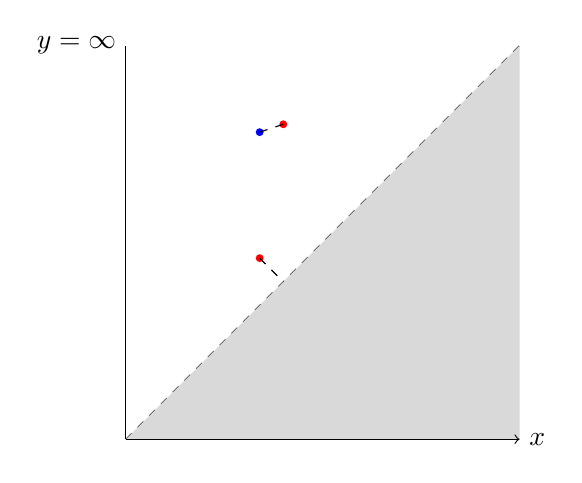
\begin{tikzpicture}
  \draw[dashed] (0, 0) -- (5, 5);
  \fill[gray!30] (0, 0) -- (5, 5) -- (5, 0) -- cycle;
  \draw[->] (0, 0) -- (5, 0) node[right] {$x$};
  \draw[-] (0, 0) -- (0, 5) node[left] {$y=\infty$};
  \fill[red] (1.7, 2.3) circle (0.05);
  \fill[red] (2, 4) circle (0.05);
  \fill[blue] (1.7, 3.9) circle (0.05);

  \draw[dashed] (2, 4) -- (1.7, 3.9);
  \draw[dashed] (1.7, 2.3) -- (2, 2);
\end{tikzpicture}
\caption{Barcodes matching on a persistence diagram}
\label{fig:persistence diagram domaine}
\end{figure}

\begin{proof}
  Let $f, g : X \to \R$ be 2 tame functions. We denote $\varepsilon = \|f-g\|_\infty$.
  We pose $F_t = f^{-1}((-\infty, t]), G_t = g^{-1}((-\infty, t])~(t\in \R)$.

  Key observation: $\left\{F_t\right\}_{t \in \mathbb{R}}$ and $\left\{G_t\right\}_{t \in \mathbb{R}}$
  are $\varepsilon$-interleaved w.r.t. inclusion:\\
  $$
  \forall t \in \mathbb{R}, G_{t-\varepsilon} \subseteq F_t \subseteq G_{t+\varepsilon}
  $$

  We denote
  $F^{2 \varepsilon}=\left\{F_{2 n \varepsilon}\right\}_{n \in \mathbb{Z}}$,
  $G^{2 \varepsilon}=\left\{G_{2(n+1) \varepsilon}\right\}_{n \in \mathbb{Z}}$
  2 discret filtrations.
  $$
  \cdots \subseteq F_0 \subseteq G_{\varepsilon} \subseteq F_{2 \varepsilon} \subseteq \cdots \subseteq G_{(2 n-1) \varepsilon} \subseteq F_{2 n \varepsilon} \subseteq G_{(2 n+1) \varepsilon} \subseteq \cdots
  $$
  We denote another discret filtration $\left\{H_{n \varepsilon}\right\}_{n \in \mathbb{Z}}$, where $H_{n \varepsilon}=\left\{\begin{array}{l}F_{n \varepsilon} \text { if } n \text { is even } \\ G_{n \varepsilon} \text { if } n \text { is odd }\end{array}\right.$

  $$
  d_\infty(\Dg~f, \Dg~g) \le d_\infty(\Dg~f, \Dg~F) + d_\infty(\Dg~F, \Dg~H) + d_\infty(\Dg~H, \Dg~G) + d_\infty(\Dg~G, \Dg~g)
  \le (2+1+1+2)\varepsilon \le 6\varepsilon
  $$
  (We can optimise it to $\varepsilon$, but difficult)
  
\end{proof}